\documentclass[12pt]{book}              
%\parindent0pt  \parskip10pt             % make block paragraphs
%\raggedright                            % do not right justify

\usepackage[margin=2cm]{geometry}
\usepackage{paralist}
\usepackage{url}
\usepackage{siunitx}
\usepackage{listings}
\usepackage{graphicx} 
\usepackage{booktabs} % for much better looking tables
\usepackage{array} % for better arrays (eg matrices) in maths
\usepackage{verbatim} % adds environment for commenting out blocks of text & for better verbatim
\usepackage{subcaption} % make it possible to include more than one captioned figure/table in a single float
\usepackage{float}
\usepackage[hyperfootnotes=false]{hyperref}
%\floatstyle{boxed} 
\restylefloat{figure}

\lstset{
  framexleftmargin=10mm, 
  tabsize=2,
  language=c, 
  frame=single,
  numbers=left,
  keepspaces,
  basicstyle=\footnotesize,
%  basicstyle=\small\ttfamily,
}


\title{CPSC 1000 - Laboratory manual}    % Supply information
\author{Robert Benkoczi}              %   for the title page.
\date{\today\\ version 3.1.1}  %   Use current date. 

%\renewcommand{\chaptername}{Activity}

% Note that book class by default is formatted to be printed back-to-back.
\begin{document}                        % End of preamble, start of text.
\frontmatter                            % only in book class (roman page #s)
\maketitle                              % Print title page.
\tableofcontents                        % Print table of contents

\chapter{License}



\includegraphics[width=4em]{by-sa.png}

\noindent
This laboratory manual is licensed under a Creative Commons
Attribution-ShareAlike 4.0 International License.

\noindent
\url{http://creativecommons.org/licenses/by-sa/4.0/}

\chapter{Introduction}

This manual accompanies the lab activities for course CPSC 1000,
Introduction to Computer Science, offered at the University of
Lethbridge. In this offering of the course, the students learn to
make simple projects using the Arduino micro-controller. 

The first part of this manual concentrates on four basic functions of
a micro-controller: reading digital and analog signals, and generating
digital and analog signals. Then, in Part 2, the students start
working on a larger project that involves controlling the movement of
a simple three wheel robotic gadget and making it autonomous to some
degree.

Students who complete the activities in this manual will have a basic
understanding of how to program an Arduino micro-controller and will
posses some elemental knowledge concerning simple electronic
components such as resistors, light emitting diodes, various sensors,
and direct current motors. They will be ready to learn about other, more
advanced electronic components and how to build more complex projects.

\paragraph{Suggested lesson plan:} This course was offered at the
University of Lethbridge during a twelve week semester. Every week,
students participated in a two hour lab session and 150 minutes of
lectures. For Part I, a format for lectures and lab sessions that
seems to have worked well was the following:
\begin{compactitem}[--]
  \item Lectures held during a week introduced the background
    necessary for the lab activity taking place the following
    week. The labs started in week two, so there were only 11 weeks of
    lab activities.
  \item Lab sessions, the first 45 - 60 minutes of the two hour long
    session: the lab instructor demonstrated the activity described in
    this manual and each student, individually, followed the
    instructions in order to complete the activity.
  \item Lab sessions, the remaining time: after the activities were
    completed, the students were assigned one or more exercises from
    the lab manual and were given marks for completing them.
\end{compactitem}

For Part II of the course, the students were paired in teams and were
asked to complete the three challenges described in Part II of this
manual. The lectures were moved from the standard classroom into the
lab and were converted to lab sessions. Instructors provided guidance
and help as needed, but the students were expected to work on their
challenges at their own pace.

The twelve weeks of the semester were allocated to the activities as
follows.
\begin{compactitem}
\item[Week 1:] Activity 0 (Chapter \ref{activity0.se}) and general
  concepts for lectures, input/output. No labs.
\item[Week 2:] Activity 1 (Chapter
  \ref{lab1.ch}) for lectures, functions and variables. Activity 0 for labs.
\item[Week 3:] Activity 2 (Chapter \ref{se:pot}) for
  lectures, expressions. Activity 1 for labs.
\item[Week 4:] Activity 3 (Chapter \ref{ch2.chap}) , pull-up/pull-down
  resistors for lectures. Activity 2 for labs.
\item[Week 5:] Activity 3 (c'ed), selection statements for
  lectures. Activity 3 for labs.
\item[Week 6:] Activity 4 (Chapter \ref{se:ch4}) for lectures, PWM,
  loops. Activity 3 (c'ed) for labs.
\item[Week 7:] Activity 5 (Chapter \ref{ch:ex5}) for lectures. Activity
  4 for labs.
\item[Week 8:] Software engineering concepts in lectures. Activity 5
  for labs.
\item[Weeks 9-12:] Lab activities only, students complete the project
  challenges. 
\end{compactitem}

\paragraph{Editing this manual:} This manual is written in
\LaTeX. Figure \ref{fig:2eyes} was created using the XFig vector
drawing program (see
\url{http://mcj.sourceforge.net/installation.html}), which is
available on most linux distributions. The circuit diagrams were
created with Autodesk Eagle (see
\url{https://www.autodesk.com/products/eagle/free-download}), for
which a free version is available for download.

\paragraph{Code:} The source code listings in this manual are
extracted from the Arduino source files located in subdirectory \emph{src} in
the source directory of this manual. These programs can be compiled
and uploaded onto the Arduino board. 

\paragraph{Acknowledgements:} 
I have many people to
thank for their contribution to making this manual better: my CPSC
1000 class of Spring 2018, who used it in the first offering; my
excellent team of graduate student lab instructors: Aryal Chudamani,
Tanvir Fuad, Adam Lefaivre, Nicholas Parsons, and Mainul Polash; my
graduate student Nicholas Parsons who drew the circuit diagrams,
wrote the initial version for most of the Arduino code, and
implemented almost all of the activities in this manual to make sure
the information provided here is accurate; and last but not least, my
colleague Nicole Wilson, for valuable advice and feedback on
this material. 


\mainmatter                             % only in book class (arabic page #s)

\part{Fundamental concepts}

\chapter{Activity 0: Arduino and its programming
  language}\label{activity0.se} 

\section{Lab activity objectives}\label{lab0obj.se}

An Arduino micro-controller is essentially a special kind of
computer. It is a computer with a very limited ``user
interface'', because a micro-controller is not supposed to be
handled directly by humans. It is designed to interact with other
electronic components.

In this activity, students will interact with an Arduino
micro-controller using the Arduino IDE computer program as an
intermediary. Students will upload code onto (or program) an Arduino
  micro-controller and will learn some basic programming commands that
  will allow the Arduino to perform operations like any other
  computer.

\section{Component list}
\begin{compactitem}[--]
  \item 1 x Arduino micro-controller
  \item 1 x USB cable
\end{compactitem}


\section{Circuit set-up}\label{se:setup0}

For this activity, no electronic circuit is really necessary. Simply
connect the USB cable to the Arduino board and then connect the other
end of the cable into the USB port of your workstation, thus powering
up the Arduino.

The USB cable will be used to provide power to the device and to
transmit information back and forth between the micro-controller
and the workstation. 

\section{Arduino program}

An Arduino program contains two mandatory functions that must be
defined by the programmer: 
\begin{inparaenum}[(1)]
\item Line 1: \emph{setup}, which is executed a single time when the
micro-controller is powered up or when the code is uploaded to the
Arduino, and 
\item Line 6: \emph{loop} which is executed repeatedly, for as long as the
Arduino is powered up and no other program is uploaded.
\end{inparaenum}
The instructions to be executed by \emph{setup} and \emph{loop} must
be inserted in the body of these functions, namely between \{ and \}. 

\lstinputlisting[caption={Arduino code for Activity 0: Output ``Hello
    world''},label=lst:ex0,
  firstline=8]{src/exp0_hello.ino}

\begin{compactitem}[--]
  \item Line 3: Since the Arduino has a very limited user interface,
    we will use the workstation and the \emph{Serial Monitor}
    application to interact with the micro-controller via the USB
    cable. In line 3, the command initializes the speed of the serial
    communication on the cable. The same speed must be selected in the
    Serial Monitor application.

    \item Line 4: the command
      \texttt{Serial.println} outputs messages that can be received
      and displayed by the Serial Monitor.
\end{compactitem}


\section{Instructions}

\begin{compactitem}[--]
\item Start the Arduino IDE application on the workstation. Open the
  Serial Monitor Window and check that the speed of the serial port is
  set to 9600.

\item Make sure the Arduino is connected to the workstation via the
  USB cable. Upload the program on the Arduino.

\item You should see the ``Hello world'' message in the serial monitor
  window.

\item Add a \texttt{Serial.println} command in the body of function
  \texttt{loop} (on line 7, between \{ and \}) to output message
  ``Hello again''. Please observe the specific syntax of the command:

  \lstinline{Serial.println ( message ) ;}

  The parenthesis and semicolon are mandatory. 
  Upload the modified program. What do you notice?

\item The command \lstinline$delay(value);$ instructs the
  micro-controller to take a pause of a specified number of
  milliseconds. That is, the following instruction will be executed
  after the given number of milliseconds (value) have passed. This
  number must be provided in the command, between the parenthesis. For
  example, \lstinline$delay(200);$ creates a pause of 200
  milliseconds. 

  What value should be given to the command to create a pause of 1
  second? If you are required to output the message ``Hello again''
  only once every second, where would you insert the command in the
  Arduino code?

  Implement the change and run the program.

\item A computer is sometimes used to perform calculations. For
  example, the Arduino can be used as a basic calculator. For example,
  the following piece of code outputs the product of 7 and 8:

  \begin{lstlisting}
    void setup() {
      Serial.begin(9600);
      Serial.println(7*8);
    }
  \end{lstlisting}

  The basic arithmetic operations are +, -, *, /, and \% (sum,
  difference, product, division, and modulus).

  Create a new Arduino project with no commands for the loop function
  but with the appropriate command to set-up the speed of the serial
  communication module (see the sample code above). Write code that
  outputs the perimeter of a rectangular room with sides 12 and 17
  feet. Use the arithmetic operations.

\item Some mathematical operations are available as functions. For
  example, computing $a^b$ for some numerical values $a$ and $b$ is
  achieved using function \texttt{pow}:

  \lstinline$pow(a, b);$
  
  Information about the Arduino functions is available at
  \url{https://www.arduino.cc/reference/en/#functions}. Using
  this reference, modify your code to display
  $\sqrt{3.14}$. Then, write another println command that computes
  $3.14^\frac{1}{2}$.  
  
\item A computer program has the ability to represent and store data,
  using variables. For example, we can store numerical values in
  variables and we can perform numerical computations on those
  variables.

  Variables are locations in memory that have a name. To create such a
  location, we need to \emph{define} or \emph{declare} the
  variable. 

  The code \lstinline$int a;$ defines a variable with the name ``a''. Variable
  ``a'' can hold integer values (\lstinline$int$). Other types of
  values are \lstinline$byte$ (integers between 0 and 255),
  \lstinline$long$ (integers from $-2^{31}$ to $2^{31}-1$),
  \lstinline$float$ (decimals between approximately $-3.4 \times
  10^{38}$ to $3.4 \times 10^{38}$), and \lstinline$String$ (text).

  The following program declares a \emph{global} integer variable with
  the name ``x''. The code, otherwise does not use the
  variable. Notice that the variable is declared outside of the
  functions loop and setup!

  \begin{lstlisting}
    int x;

    void setup() {
      Serial.begin(9600);
    }

    void loop() {
    }
  \end{lstlisting}

  To do: modify your existing code (or start a new project if you
  prefer). Then, write the code given above. Compile the project to
  see if it compiles correctly. Declare a second variable that can
  hold decimals with the name ``f''.

  \item To be used, variables need to be initialized or given a
    value. When declaring a variable, we can also initialize it. For
    example, we can declare and initialize variable ``x'' to zero:

    \lstinline$int x=0;$

    Modify your code to declare and initialize ``x'' to zero and ``f''
    to 1.5.

  \item Once initialized, variables can be used in calculations or
    they can be displayed on the serial monitor in the same way we
    displayed expressions or calculations. Examples:
    
    \lstinline$Serial.println(x);$

    \lstinline$Serial.println((x+7)/2);$

    These examples must be written in the body of functions. Write in
    your code the instruction to display the value of ``x'' in the
    body of function \emph{loop}. Add also the appropriate delay
    command so that the value is displayed only once every second.

  \item The advantage of a variable lies in the ability to change the value
    stored by the variable. We use the operator ``='' to assign new
    values to the variable. This operation is called
    \emph{assignment}. Examples:

    \lstinline$x = 1;$

    \lstinline$x = x + 1;$

    The last command increases the value of the variable by one, and
    it is a very common operation for programmers.

    The syntax of the assignment operation is as follows:

    \underline{variable to
      be modified} = \underline{expression for the new value} ;

    Modify your code so that you increase the value of variable ``x''
    by one after you display the value of ``x'' in the loop function.
    Compile and upload the code.
\end{compactitem}

Congratulations. You are now familiar with the the basic instructions
for an Arduino program. More information is available from the Arduino
Notebook by Brian Evans, available from the course web page.


\section{Exercises}

\begin{enumerate}[1.]
\item Write Arduino code that displays on the Serial monitor a count
  down from 1000, every second. Example: the counter displays first
  1000, then 999 after 1 second, then 998, etc.

\item Reduce the time between successive counts for the count down
  counter to half a second.

\item (*) Using only arithmetic expressions, create an Arduino program
  that displays two counters one after the other. The
  first counter increases by one every second, the second increases by
  one every 10 seconds. For example, the program should display 0 0,
  then after a second 1 0, then 2 0, ..., 9 0, 10 1, 11 1, ... 19 1,
  20 2, etc. 
\end{enumerate}


%%%%%%%%%%%%%%%%%%%%%%%%%%%%%5

\chapter{Activity 1: blinking led (digital output)}\label{lab1.ch}

\section{Lab activity objectives}\label{lab1obj.se}

Digital data is binary data or data represented by 1-s and 0-s. The
hardware of a computer encodes 1-s and 0-s for example, using the
presence or absence of voltage. In this session, students will learn how an Arduino
micro-controller outputs digital information on its digital pins, how
bits\footnote{\textbf{bi}nary digi\textbf{ts}} are represented,
and how we can use the voltage that represents digital information to
turn a LED on. Digital output has many uses in practical systems. For
example, the digital output from an Arduino micro-controller can
control sensors, such as the cheap ultrasonic distance
sensor HC-04. The circuit with LED described here illustrates the
steps needed to work with digital output in a simple and direct way. 

 In this session, students will:
\begin{compactitem}[--]
\item use the Arduino IDE\footnote{Integrated Development Environment}
  application to upload a simple program to an Arduino
  micro-controller,
\item recognize the polarity of a LED\footnote{Light Emitting
    Diode},
\item connect a LED, resistor, and Arduino using wires and a
  breadboard\footnote{A breadboard is used to create circuits that can
    be easily reconfigured using wires (see
    Fig.~\ref*{fig:breadboard}).} according to a given circuit diagram, 
\item extend the circuit by adding a second resistor and LED, and
  extend the Arduino program to perform a new function,
\item draw the diagram for the new circuit.
\end{compactitem}

\section{Component list}
Including the components necessary for the exercises, the following
parts are needed:
\begin{compactitem}[--]
  \item 1 x Arduino micro-controller
  \item 1 x USB cable
  \item 1 x breadboard
  \item 5 or 6 M-M jumper wires of assorted length
	\item 2 x 220 Ohm resistor
	\item 2 x LED
\end{compactitem}

\section{Circuit set-up}\label{se:setup1}

\begin{compactitem}[--]
  \item Select the breadboard from the component box and examine the
    circuit diagram from Fig.~\ref*{fig:SchemEx1}. Using some of the
    jumper wires and the breadboard, you will set-up the circuit in
    the diagram, as follows.
	\item Select one LED from the component box and identify
    the polarity of its pins (see
    Fig.~\ref*{fig:diode}). The LED works only if inserted in the
    correct polarity according to the diagram. Insert the LED into the
    breadboard, making sure its pins are inserted in different rows on
    the breadboard (why?).
	\item Select one resistor from the component box. Insert one pin of
    the resistor on the row containing the LED cathode. The resistor can
    be inserted in any direction. Insert the other pin of the resistor
    to the negative breadboard power bar (the power bars are marked by
    red arrows in Fig.~\ref*{fig:breadboard}).
  \item Use a jumper wire to connect the row containing the LED anode
    to digital pin 13 (D13) on the Arduino. Use another jumper wire to
    connect the Arduino GND pin to the negative breadboard power bar
    containing the pin of the resistor (the two negative/positive 
    power bars on the breadboard are not interconnected).
\item The circuit from Fig.~\ref*{fig:SchemEx1} is now complete.
\end{compactitem}


\begin{figure}[tb]
	\centering
  \begin{subfigure}[b]{0.55 \textwidth}
	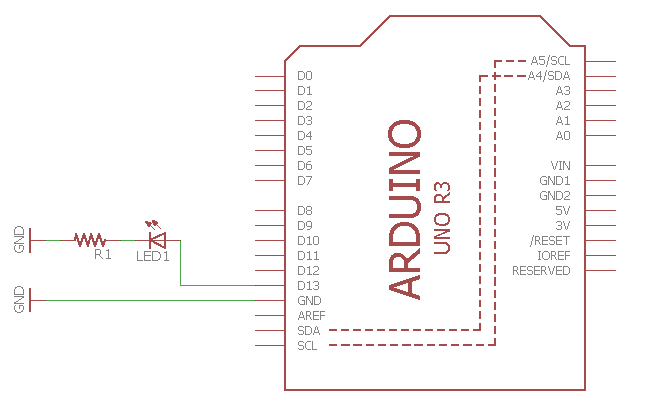
\includegraphics[width=\textwidth]{schem/Experiment1}
	\caption{Circuit diagram for Activity 1}
	\label{fig:SchemEx1}
  \end{subfigure}
\hfill
  \begin{subfigure}[b]{0.4 \textwidth}
  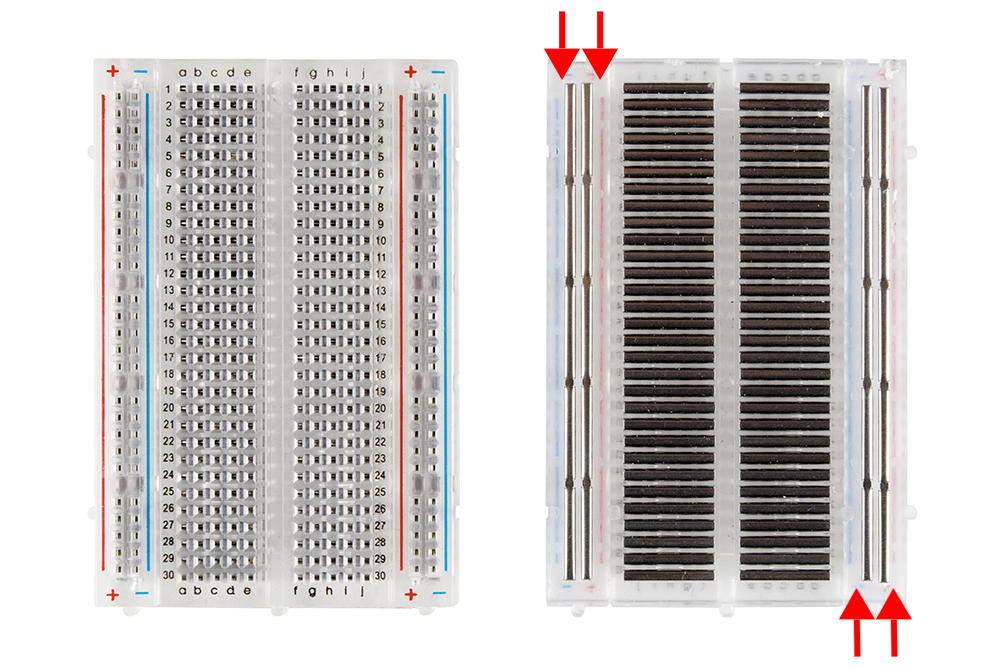
\includegraphics[width=\textwidth]{schem/breadboard.jpg}
  \caption{Breadboard internal connections, source \url{learn.sparkfun.com}}
  \label{fig:breadboard}
  \end{subfigure}\\
\vspace*{.5em}
\begin{subfigure}{0.5\textwidth}
\centering
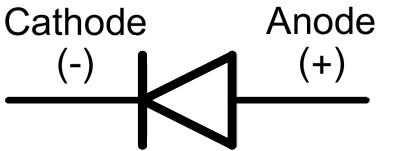
\includegraphics[width=0.5\textwidth]{schem/diode-schema.png}\\
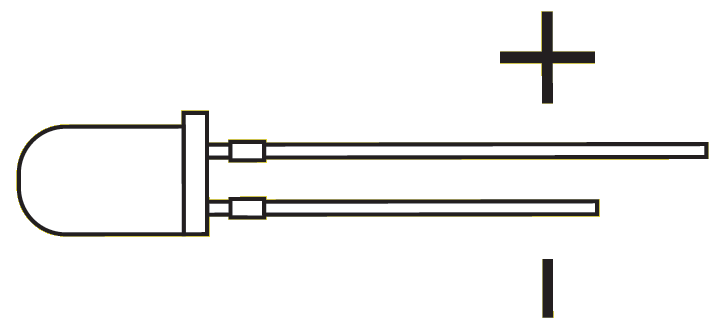
\includegraphics[width=0.5\textwidth]{schem/diode-part.png}
\caption{Polarity of a LED, source \url{learn.sparkfun.com}}
\label{fig:diode}
\end{subfigure}
\caption{Circuit set-up}
\label{fig:setupA1}
\end{figure}


\section{Arduino program}

\begin{compactitem}[--]
\item Line 3: an Arduino has digital and analog pins (which we will
  examine in future activities), and the digital pins can be
  configured to either read digital information (input), or output
  digital information. On line 3, we tell Arduino to use its pin
  number 13 for output. 
\item Line 8: in output mode, the digital pin can be either in HIGH
  mode, representing bit 1, or low mode, representing bit 0. In this
  case, we set the pin to output bit 1. This 
  information is encoded by a certain voltage present on the
  pin. Exercise \ref*{ex:measure} asks you to determine the voltage
  encoding this information. 
\item Line 10: we set pin 13 to output bit 0.
\item Lines 9 and 11: we ask the Arduino board to pause, which means
  that the command following function \emph{delay} will only be
  executed after 1000 milliseconds (1 sec) have passed (see Chapter
  \ref{activity0.se}). 
\end{compactitem}

\lstinputlisting[caption={Arduino code for Activity 1},label=lst:ex1, firstline=21]{src/exp1_blink.ino}


\section {Instructions}

\begin{compactitem}[--]
\item Assemble the circuit according to the instructions from Section
  \ref{se:setup1}. 
\item Connect the Arduino to your computer using the USB cable from
  the component box. The Arduino micro-controller is powered by the
  computer, via the USB cable. This power is sufficient to light a few
  LEDs, but for more energy hungry components such as motors, we will
  need a different set-up.
\item Start the Arduino IDE on the computer. Navigate to the
  \emph{Tools/Ports} menu and select the port with a description
  containing the name ``Arduino''. Ensure that \emph{Tools/Board} is
  set to ``Arduino/Genuino Uno''. 
\item Navigate to the \emph{File} menu and load the lab code provided
  by the instructor. Convince yourself that the code displayed matches
  Listing \ref*{lst:ex1}.
\item  Compile and upload the code to the Arduino by clicking
the arrow icon on the toolbar.  The
check-mark icon to the left will compile the sketch
without uploading it to the Arduino. This is useful for checking that
your program is syntactically correct. It is a good idea to save frequently,
compile early, and compile often. 

\item Once the IDE has completed the upload, the circuit LED should now be flashing. 
\end{compactitem}

\section{Exercises}

\begin{enumerate}[1.]
\item\label{ex:measure} Use a voltmeter to determine the voltage
  representing bit 1 and the voltage representing bit 0 in an Arduino
  circuit.

\item Change the Arduino program so that the LED stays on for 2
  seconds and off for 1 second.

\item Change the Arduino program so that the LED blinks 4 times in a
  second.

\item\label{ex:two} Extend the circuit to add the second LED and
  resistor in such a way that the two LEDs can be independently turned
  on or off. 
\begin{compactenum}[(a)]
\item Make a drawing of your new circuit.
\item Extend the Arduino code so that your circuit blinks the two LEDs,
  alternatively, using a pattern similar to that of the lights at a
  railway crossing. Set the delays so that each LED is on for one
  second and off for one second.
\end{compactenum}

\item Modify the code from Exercise \ref*{ex:two} to implement
  different blinking patterns, for example one LED blinks twice as
  fast as the other, or both LEDs blink at the same time and with the
  same frequency, or both LEDS blink with the same frequency but one
  LED starts 250 milliseconds after the other, etc.
\end{enumerate}


%%%%%%%%%%%%%%%%%%%
\chapter{Activity 2: potentiometer (analog input)}\label{se:pot}

\section{Lab activity objectives}

Many sensors provide information via an analog signal, more exactly
via a voltage that can take any value between 0V and 5V. In this
activity, students will program the Arduino board to read the variable
voltage obtained over the pins of a variable resistor or
potentiometer. The value will be sent, via the USB
cable, to the host computer to be
displayed. More precisely, the students will:
\begin{compactitem}[--]
\item identify the pins of a variable resistor,
\item assemble a circuit using the variable resistor,
\item program the Arduino board to measure the voltage of an analog
  signal using the Arduino's analog pins,
\item program the Arduino to send the value read from the analog pin,
  over the serial USB connection, to the workstation,
\item open the serial monitor window in the Arduino IDE on the 
  workstation to view the value read by the analog pin.
\end{compactitem}


\section{Component list}

Including the components necessary for the lab assignment, the following
parts are needed:
\begin{compactitem}[--]
  \item 1 x Arduino micro-controller
  \item 1 x USB cable
  \item 1 x breadboard
  \item 8 or 10 M-M jumper wires of assorted lengths
	\item 1 x 220 Ohm resistor
	\item 1 x LED
  \item 1 x 10k Ohm Variable Resistor (Potentiometer)
\end{compactitem}


\section{Circuit set-up}

The circuit set-up is very simple for this activity. We need to
identify the pins on the potentiometer first. The resistance between
the middle pin and one of the outer pins is variable. The connection
in Fig.~\ref*{fig:SchemEx3} can be interpreted as two series connected
resistors for which the sum of their electrical resistance is constant
and equals 10 k Ohm, but each resistor has a variable resistance. This
way, the current from the +5V pin to the GND pin on the Arduino is
limited, but the voltage over the resistors is variable. We are
measuring on Analog pin 1 the voltage over one of the resistors and we
output this value by communicating it to the host computer which will
display it.

\begin{figure}[tb]
	 \centering
	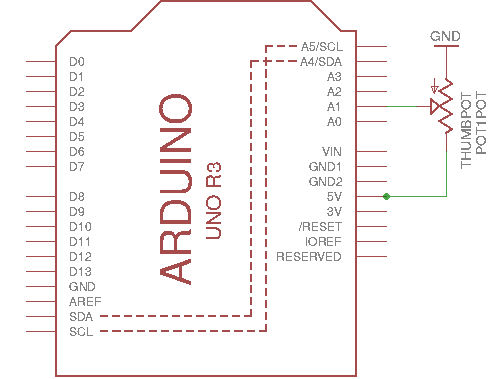
\includegraphics{schem/Experiment2}
	\caption{Circuit set-up for Activity 2}
	\label{fig:SchemEx3}
\end{figure}

\section{Arduino program}

The short program demonstrates the use of serial communication (see
Chapter \ref{activity0.se}, and commands for reading the voltage applied to an
analog pin on the Arduino.

\begin{description}
\item[Serial communication:] the syntax appears slightly particular,
  as function calls are prefixed by the identifier
  \lstinline$Serial$, which identifies the so called serial port,
  followed by period and the function name. The port
  \lstinline$Serial$ is used for the connection via the USB cable, and
  depending on the type of the Arduino board, other physical connections may be
  available, such as \lstinline$Serial1$, etc. In this document, we will only use
  \lstinline$Serial$. 

  To initialize the serial port, we must first call function
  \lstinline$begin$ which needs one integer argument that specifies
  the speed of communication, namely how many symbols per second to
  transmit. This speed is known as the baud rate. In Listing
  \ref*{lst:ex3}, line \ref*{a3:begin}, we use the typical rate of
  9600 baud. At the other end of communication, we must configure the
  serial monitor of the Arduino IDE running on the workstation to use
  the same speed value, 9600 baud (see Chapter \ref{activity0.se}).

  On line \ref*{a3:println} we output the numeric value provided as
  argument to the serial monitor window of the Arduino IDE running on
  the workstation. 
\item[Analog input:] The six analog pins numbered from $0$ to $5$ are
  only capable of input. Function \lstinline$analogRead$ returns an
  integer in the range $0$ to $1023$, where integer $0$ corresponds to
  a voltage of $0$ V on the analog pin, and value $1023$ corresponds
  to the maximum voltage of $5$ V that can be measured on the pin. The
  function argument is an integer from $0$ to $5$ that identifies the
  pin used for input.
\end{description}

The last command in function \lstinline$loop$ is a call to the delay
function. We do not need to sample the voltage on the analog pin too
frequently. 

\lstinputlisting[caption={Arduino code for Activity 2 (potentiometer)},label=lst:ex3,escapechar=|,firstline=12]{src/exp2_analog.ino}


\section{Instructions}

\begin{compactitem}[--]
\item Assemble the circuit in Fig.~\ref*{fig:SchemEx3}.
\item Start the Arduino IDE program and select the appropriate port
  for the Arduino board as in the previous activities.
\item Select menu Tools, then Serial Monitor. In the window that
  opens, make sure that 9600 baud is selected from the pull down widget.
\item Download the starting code provided by the instructors and
  upload it. The serial monitor should display the value read from Analog
  pin 1, every 500 ms.
\item Turn the knob on the potentiometer and observe how the value
  shown by the serial monitor changes.
\end{compactitem}

\section{Exercises}\label{exercises:ch3}

\begin{enumerate}[1.]
\item The value of the resistance between the outer pins on the
  potentiometer is 10 k Ohm. Calculate the value of the current
  flowing from pin +5 to GND on the Arduino. As one turns the
  potentiometer knob changing the voltage applied to the analog pin,
  do you expect that the value of the current will change? Explain.

\item Suppose we change the circuit from Fig.~\ref*{fig:SchemEx3} by
  moving the connector from pin +5V to pin +3V on the Arduino. What is
  the range of values that are likely to be returned on the Serial
  monitor in this case? You may assume that integer values are
  assigned uniformly in the range $0$ V to $5$ V.

\item\label{ex3:ch3} Add an LED and a 220 Ohm resistor to the circuit from
  Fig.~\ref*{fig:SchemEx3} and connect the LED to one of the digital
  pins in the range 2 to 13 (pins 0 and 1 are used during the
  transmission of data over the serial link). Copy the \emph{blink}
  function from the sample code provided on Moodle for lectures into
  the code from Listing \ref*{lst:ex3}. Adjust the code so that the
  duration the LED is on or off equals to the value read by the analog
  pin in milliseconds (the LED
  should be on for a time equal to the value read in milliseconds,
  and off for an equal amount of time). Your program should continue
  to send the value read by the analog pin to the serial monitor.

\item Add two LED's to the  circuit from
  Fig.~\ref*{fig:SchemEx3}, and arrange them so that one LED is on the
  left, the other on the right. Program the Arduino so that when the
  voltage measured by the analog pin is in the range $0$V to $2$V, the
  left LEDs is on and the right one< is off. When the voltage is between
  $3$V and $5$V, the right LED is on and the left is off. When the
  voltage is between $2$V and $3$V, both LEDs should be on.
\end{enumerate}



%%%%%%
\chapter{Activity 3: push button (digital input)}\label{ch2.chap}

\section{Lab activity objectives}\label{se:obj2}

Any interesting Arduino project should allow for some user input. The
simplest way for a user to interact with an Arduino project is through
buttons. 
In this lab activity, we investigate a circuit set-up and the
corresponding Arduino program that allows the micro-controller to read
the state of a momentary button\footnote{A momentary button closes the
  circuit, or connects the two terminals together, for as long as the
  button is pressed.} which can be either in pressed or depressed state. The circuit we use is a
standard one using a so called \emph{pull-up resistor}. A pull-up
resistor  connects the input pin on the Arduino to +5V when the button is
not pressed (bit 1) and to 0V when the button is pressed (bit 0). By
reading the input pin, the micro-controller determines the state of
the button. 

In this session, students will:
\begin{compactitem}[--]
\item use a breadboard, an LED, and resistors to examine the wiring of
  the push button and to determine which pins on the button become connected when the
  button is pressed, 
\item use a breadboard to create a pull-up circuit for the Arduino using a
  resistor and the push button,
\item combine this circuit with the circuit from Chapter
  \ref{lab1.ch} so that pressing the button will change the state of
  the LED as follows.
\begin{compactitem}[-]
\item Initially, the LED is off.
\item When the button is pressed, the state of the LED is toggled: if
  the LED is off, it will be turned on, and if it is on, it will be
  turned off. 
\end{compactitem}
\item use appropriate delay values in the Arduino program to read the
  state of the button reliably. 
\end{compactitem}


\section{Component list}

A few of the exercises at the end of this lab require additional components that what is strictly necessary for the activities proposed. The following
parts are needed:
\begin{compactitem}[--]
  \item 1 x Arduino micro-controller
  \item 1 x USB cable
  \item 1 x breadboard
  \item 8 or 10 M-M jumper wires of assorted lengths
	\item 2 x 220 Ohm resistor
	\item 2 x LED
  \item 1 x 10k Ohm Resistor (Pull-up)
  \item 1 x push button
\end{compactitem}


\section{Circuit set-up}\label{se:setup2}

Use the breadboard and the supplied parts to assemble the circuit from
Fig.~\ref{fig:SchemEx2}. Please take note of the identity of the Arduino
pins used. The sample program is written on the assumption that pin D2
is connected to the push button and pin D13 is connected to the LED.

The supplied push button has four pins that can be inserted in the
breadboard. Two of the four pins are inter-connected internally. The
other two are inter-connected as well. See Fig.~\ref{fig:button} to identify
the pins that are inter-connected.  When the button
is pressed, the two pairs of inter-connected pins become connected to
each other (all four pins are inter-connected). When the
button is depressed, the connections return to their initial
configuration. To be able to use the button, make sure you insert it
in the breadboard in such a way that the pair of pins that are farther
apart share the same row on the breadboard. To have room for
additional connections, the button should straddle the vertical axis
of symmetry of the breadboard. For example, the button pins should
be inserted in columns \emph{d} and \emph{g}. 

\begin{figure}[tb]
	 \centering
  \begin{subfigure}[b]{0.65 \textwidth}
	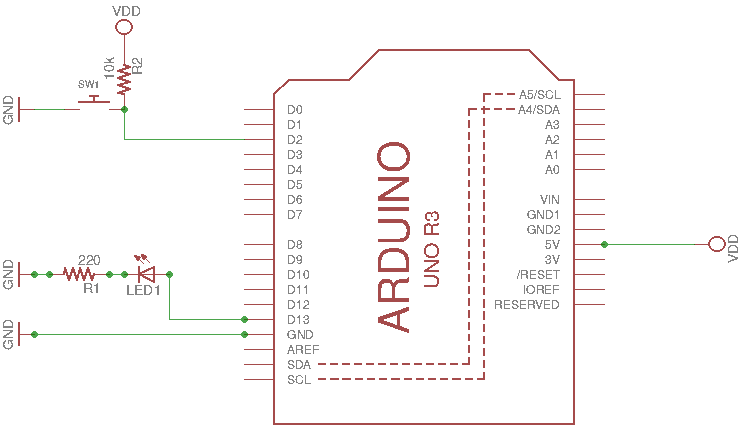
\includegraphics[width=\textwidth]{schem/Experiment3}
	\caption{Circuit diagram for Activity 3}
	\label{fig:SchemEx2}
  \end{subfigure}
\hfill
  \begin{subfigure}[b]{0.3 \textwidth}
  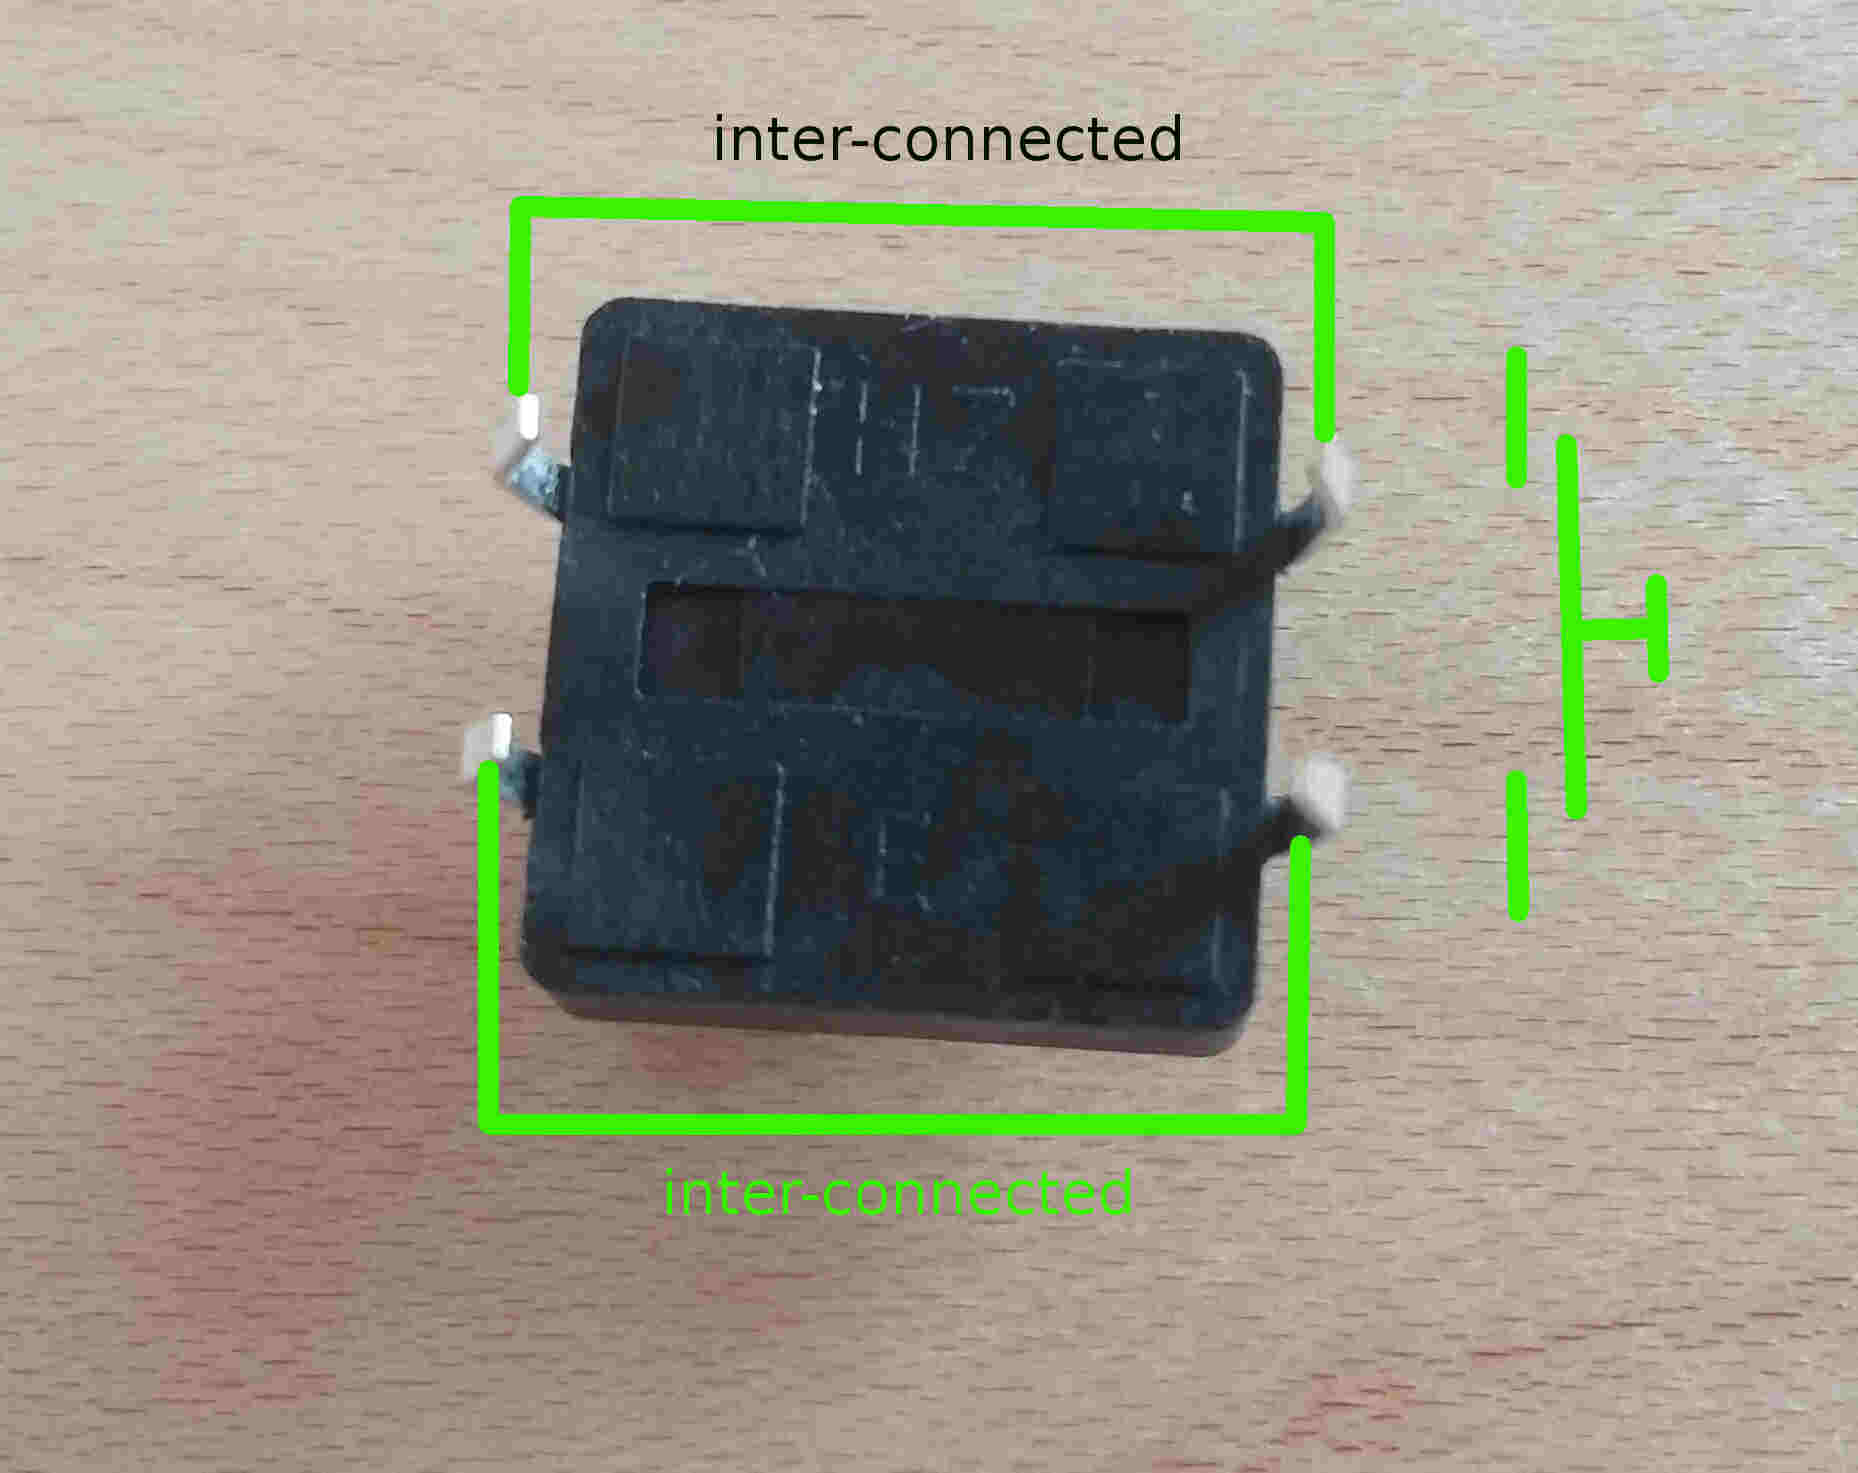
\includegraphics[width=\textwidth]{schem/button2.jpg}
  \caption{Back side of the push button and its internal
    connections}\label{fig:button} 
  \end{subfigure}
  \caption{Circuit set-up for Activity 3}\label{fig:setup2}
\end{figure}


\section{Arduino program}

Download the Arduino source code called \emph{exp3\_button.ino} from the source code folder in the lab manual section on Moodle.
In this program, we use the global variable \lstinline$LED_state$ to
remember whether the LED is on or off. We define two functions,
\lstinline$isButtonPressed$ which returns true if the button is
pressed, and \lstinline$setLED$ which accepts one argument that
specifies what state we wish the LED to be in: false for LED off and
true for LED on. Line \ref*{a2:toggle} is responsible for the logic of
this program: the state of the LED changes from continuously on to
continuously off each time the button is pressed. 

Notice the delay value from function \lstinline$isButtonPressed$, which
ensures that we do not read the state of the input pin too frequently,
but also not too infrequently so that we miss most of the button
presses. In function \lstinline$loop$, the larger delay value ensures
we do not immediately read the state of the button to change the state
of the LED again. 

Consider what happens if we keep the button pressed. How about if we
change the delay values in the code significantly? How about if we do
not have delay values at all? Try to modify the code, if you have time
during the lab, to investigate these questions.

\lstinputlisting[caption={Arduino code for Activity 3 (push button)},label=lst:ex2,escapechar=|,firstline=10]{src/exp3_button.ino}

\section{Instructions}

\begin{compactitem}[--]
\item Assemble the circuit according to the instructions from Section
  \ref{se:setup2}. Verify that you are using the correct resistors in
  the connections and that you are inserting the button in the
  breadboard correctly. 
\item Connect the Arduino to your workstation using the USB cable,
  open the Arduino IDE, and load the sample code provided by the
  instructor. 
\item Upload the code and test the behaviour of the circuit.
\item Complete the lab assignment given by the instructor.
\end{compactitem}

\section{Exercises}

\begin{enumerate}[1.]
\item The Arduino board has built-in pull-up resistors for its digital
  pins. Read the online documentation about how to enable the built-in
  pull-up resistor. Modify the circuit to eliminate the 10k Ohm
  pull-up resistor and change the program if needed by your new
  circuit but without changing the behaviour of the circuit.

\item\label{pb-3state} Use the circuit from
  Fig.~\ref*{fig:SchemEx2}. Modify the program so that the LED has
  three possible states: continuously on, continuously off, and
  blinking with a frequency of 5 blinks per second. Pressing the
  button should now change the state of the LED among these three
  states.

\item Assemble the circuit from Fig.~\ref*{fig:SchemEx2} and load the program from
  Listing \ref*{lst:ex2}. Add a second button. Change the program so
  that the button is blinking continuously with a frequency of 1 Hz (1
  blink per second). Pressing one of the button should increase the blinking
  frequency by 1 Hz and pressing the other should decrease the
  frequency by 1 Hz. For simplicity, consider that the minimum
  frequency is 1 Hz.

\item\label{pb-sensor} Start with the circuit from
  Fig.~\ref*{fig:SchemEx2}. Add one 
  light sensor brick or one sound sensor brick to your design (connect
  the + or V pin on the sensor to 5V pin on the Arduino, the - or G
  pin on the sensor to the GND pin on the Arduino, and the S pin on
  the sensor to one of the analog pins on the Arduino, like
  demonstrated in the lecture). Then extend the program from Exercise
  \ref{pb-3state} so that the state of the LED changes between the
  three states when the button is pressed AND also when the sensor
  detects a change in the environment. Ideas for environment
  conditions that can trigger LED state changes: light intensity
  increases from low (below a certain threshold) to high value (above
  the threshold), the intensity of sound is above a certain
  threshold.

\item Modify the circuit from Fig.~\ref{fig:SchemEx2} so that the button is connected with a pull-down resistor instead of a pull-up resistor. Check the lecture notes for information about pull-down resistors. Modify the code accordingly. The project should have the same functionality as described in Section \ref{se:obj2}.

\item Start with the circuit from Fig.\ref{fig:SchemEx2}. Add a second LED. Modify the program from Listing \ref{lst:ex2} so that pressing the botton will cycle the LED-s through the four states defined by the following table.
  
  \begin{tabular}{ccc}
    State & LED 1 & LED 2 \\ \hline
    0 & OFF & OFF \\
    1 & ON & OFF \\
    2 & OFF & ON \\
    3 & ON & ON
  \end{tabular}

\end{enumerate}


%%%%%%%%%%%%%%%%%%%%%%%

\chapter{Activity 4: variable LED intensity (analog output /
  PWM)} \label{se:ch4} 

\section{Lab activity objectives}

In the previous activities, we learned how the Arduino board can
process input in the form of a digital and an analog signal, as well
as how to generate a digital signal for output. The goal of this
activity is to output an analog signal. Such an operation is useful
when controlling the rotation speed of a direct current (DC) motor. We
saw from the lectures that the Arduino cannot generate a
truly analog signal (it cannot supply electricity with a voltage
that can be programmed between 0 V and 5 V). However, the speed of a DC
motor is not determined by voltage but by the energy 
transferred from the source to the motor in the unit of time (also
known as power). 

Of course, the power transferred to a resistor for example, is
proportional to the square of the voltage across the resistor, as we
might know from high school or first year physics
courses\footnote{Check's Ohm's law and the definition of electric
  power to verify that $P = \frac{U^2}{R}$, where $P$ represents
  power, $U$ voltage, and $R$ resistance.}. Pulse width
modulation (PWM) is another way to control the power transferred to a
circuit, as explained in the lecture. In this activity, students will
use the PWM capable digital pins on the Arduino to control the amount
of power transferred to an LED. They will effectively control the
light intensity of the LED. The same code and principles could apply
to controlling the speed of rotation of a DC motor, except that the
power needed by the motor is larger than the power the Arduino can
transfer. We will see in Chapter \ref{ch:ex5} that we can use an
additional board, a motor shield, which can supply the additional
power needed from a pack of four AA batteries. 

More exactly, in this activity, the students will:
\begin{compactitem}[--]
\item identify the PWM enabled digital pins on the Arduino board,
\item connect an LED to PWM capable pin 9, using a circuit identical to that from
  Chapter \ref{lab1.ch},
\item  program the Arduino to vary the pulse width of the signal
  it generates on pin 9,
\end{compactitem}

\section{Component list}

The list of components for this activity is the same as for the
activity described in Chapter \ref{se:pot}. For convenience, the
components needed for the activity and the lab assignment are enumerated
below:
\begin{compactitem}[--]
  \item 1 x Arduino micro-controller
  \item 1 x USB cable
  \item 1 x breadboard
  \item 8 or 10 M-M jumper wires of assorted lengths
	\item 2 x 220 Ohm resistor
	\item 2 x LED
  \item 1 x 10k Ohm Variable Resistor (Potentiometer)
\end{compactitem}


\section{Circuit set-up}

We first identify the digital pins capable of PWM. On the Arduino Uno,
these are pins 3,5,6,9-11. On the board, these pins are marked by
symbol
\~\ next to the pin number. The Arduino program uses pin 9, so we will
connect the LED to pin 9, taking
care of the LED polarity as in Fig.~\ref*{fig:diodeEx4} (the Arduino
pin connects to the positive pin on the LED).

\begin{figure}
	 \centering
\begin{subfigure}[b]{0.55 \textwidth}
	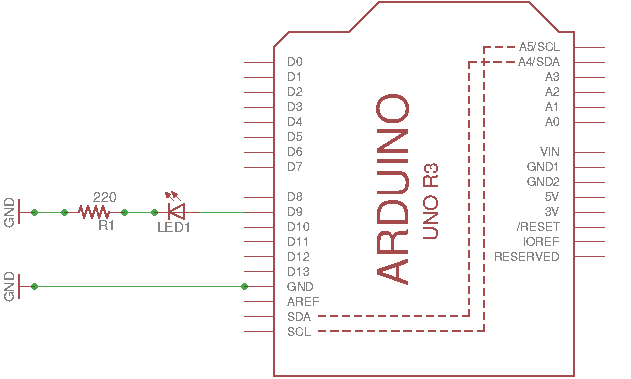
\includegraphics{schem/Experiment4}
	\caption{Circuit diagram for Activity 4}
	\label{fig:SchemEx4}
\end{subfigure}
\hfill
\begin{subfigure}[b]{0.4\textwidth}
\centering
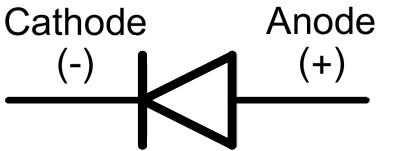
\includegraphics[width=0.5\textwidth]{schem/diode-schema.png}\\
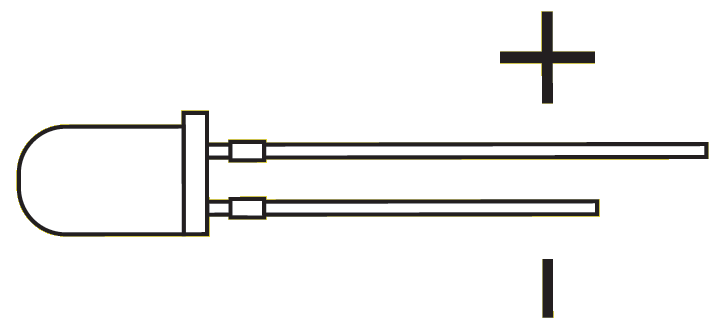
\includegraphics[width=0.5\textwidth]{schem/diode-part.png}
\caption{Polarity of a LED, source \url{learn.sparkfun.com}}
\label{fig:diodeEx4}
\end{subfigure}
\caption{Activity 4 circuit}\label{fig:main4}
\end{figure}

\section{Arduino program}

The source code in Listing \ref*{lst:ex4} demonstrates the use of one
new function.
\begin{description}
\item[analogWrite:] takes two arguments. The first, identifies the
  digital pin on which the pulse width modulated signal is output. The
  second corresponds to the amount of power transferred via the
  pin. It is an integer in the range $0$ to $255$ inclusive,
  where $0$ corresponds to no power transferred and $255$ corresponds
  to maximum power transferred. 

  We note that, to use PWM, the pin does not need to be configured in
  any special way in the \lstinline$setup$ function.
%% \item[delayMicroseconds:] takes a delay value expressed in
%%   microseconds. For this program, the goal was to fade the LED in or
%%   out from the off state to maximum intensity state in approximately 1
%%   sec. We needed thus a more accurate delay function that would
%%   maintain a certain level for the PWM signal for $\frac{1}{256}$
%%   seconds since there are 256 output levels for the PWM signal. Recall
%%   that $1000/256$ equals $3$ since the operation is performed over the
%%   integers and thus the fade in/out would last for 0.768 sec if using
%%   \lstinline$delay$. 
\end{description}

\lstinputlisting[caption={Arduino code for Activity 4 (variable LED intensity)},label=lst:ex4,escapechar=|,firstline=9]{src/exp4_dim.ino}


\section{Instructions}

\begin{compactitem}[--]
\item Assemble the circuit in Fig.~\ref*{fig:main4}. Connect the
  Arduino to the workstation via the USB cable.
\item Open the Arduino IDE, download the source code for the activity
  and open the source code in the Arduino IDE.
\item Compile and upload the program on the Arduino.
\item You should notice that the LED intensity varies in a random
  fashion, maintaining its intensity for 1 second.
\end{compactitem}

\section{Exercises}

\begin{enumerate}[1.]
\item Modify the program in Listing \ref*{lst:ex4} so that the
  intensity of the LED is assigned randomly from the range 127 to
  255. 

\item\label{gradual.ex} Using while statements, write a program that
  increases the intensity of the LED gradually from 0 to 255 in an
  interval of approximately 1 sec, then it decreases the intensity
  from 255 to 0 in the same interval of time.
  
\item Modify the program from Exercise \ref{gradual.ex} so that the LED
  stays off for 1 sec at the end of fade off, and on for 1 sec at the
  end of fade in.

\item Modify the program from Exercise \ref{gradual.ex} so that the speed
  of fade in and out is twice as slow (the LED changes from off to
  maximum intensity and vice versa within 2 sec).

\item Add a second LED to the circuit in Fig.~\ref*{fig:SchemEx4} and
  change the program from Exercise \ref{gradual.ex} so that the two LEDs
  fade in and out alternatively (one LED fades in and the other fades
  out and vice versa).

\item\label{ex4:ledpot} Add a potentiometer to the circuit in
  Fig.~\ref*{fig:SchemEx4} using the circuit from Chapter \ref{se:pot}
  as reference. Modify the code in Listing \ref*{lst:ex4} to read the
  value of the potentiometer (see Listing \ref{lst:ex3}) and to adjust the intensity of the LED as
  a function of the position of the knob on the potentiometer. More
  precisely, the LED should be off when the analog signal read is $0$
  and should have maximum intensity when the analog signal read is $1023$.  Note: the LED intensity must change immediately in response to adjusting the potentiometer (do not use \lstinline$delay()$). 

\item Extend Exercise \ref*{ex4:ledpot} with a second LED in the
  circuit. Position the LEDs in such a way that one of the LEDs is to
  the left of the other. Program the Arduino so that when the knob of
  the potentiometer is completely turned to the left, the LED on the
  left has maximum intensity while the LED on the right is
  off. Similarly, when the knob is completely turned to the right, the
  LED on the right is on and the one on the left is off. Turning the
  potentiometer on any intermediate position will modify the intensity
  of the two LEDs proportionately. 

\item Modify the program in Listing \ref*{lst:ex4} so that the
  value output by the \lstinline$analogWrite$ function is between $0$
  and $511$. What can you say about the behaviour of
  \lstinline$analogWrite$ outside the documented range of values?
\end{enumerate}

%%%%%%%%%%%%%%%%%%%%%%%

\chapter{Activity 5: variable speed DC motor (PWM via motor
  shield)} \label{ch:ex5} 

\section{Lab activity objectives}

In this Chapter, we will learn how we can use the Arduino Uno board to
control the speed of rotation of a DC motor.\footnote{A DC motor (direct
  current motor) is the simplest motor that is powered by a source of
  continuous electrical current.}
In Chapter \ref{se:ch4} we investigated how we can use the Arduino Uno
board to simulate an analog signal with pulse width modulation. This
signal was used to control the intensity of an LED. The same
principles apply to controlling the speed of DC motors, except that
the motors require more energy than what the Arduino board can supply
via its PWM signal. For this reason, our circuit will use a so called
\emph{Motor shield} which is a circuit board very much similar to the
Arduino Uno in size, but that has pins which can insert on top of the
Arduino board.
The programming of this \emph{motor shield} is also a little
different, requiring the use of a few special functions available from
the motor shield library. Instructions how to enable this library in
the Arduino IDE are available in Section \ref*{ch5:instr}.


\section{Component list}

Including the components necessary for the lab assignment, the
following parts are needed: 

\begin{compactitem}[--]
  \item 1 x Arduino Uno micro-controller
  \item 1 x USB cable
  \item 1 x Adafruit motor shield version 2.3
  \item 1 x battery holder with 4 AA batteries
  \item 2 x DC motors
\end{compactitem}

\section{Circuit set-up}

The circuit for this activity is very simple. It does not need a
breadboard. First, the motor shield needs to be inserted on top of the
Arduino Uno. There is only one orientation of the shield for which all
of the male pins on the shield are inserted in the Arduino female
slots. The circuit in Fig.~\ref*{fig:SchemEx5} shows only the
connections on the motor shield. Essentially, the DC motor needs to be
connected to the shield. In addition, the Arduino board needs to be
powered from the battery holder via the power jack. The USB cable
should also be connected to allow our programs to be uploaded.

\textbf{Important:} the Adafruit motor shield uses a jumper to
configure how the motor shield receives power. The jumper should
short-circuit the \emph{Vin jumper} pins as shown in
Fig.~\ref*{fig:SchemEx5}. This way, the shield receives power from the
Arduino board and the four AA batteries that supply it. 

\begin{figure}
	 \centering
	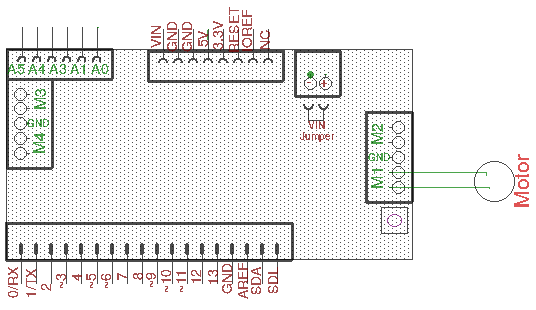
\includegraphics{schem/Experiment5.png}
	\caption{Circuit diagram for Activity 5}
	\label{fig:SchemEx5}
\end{figure}


\section{Arduino program}

The first requirement for a program that uses the Adafruit motor
shield is to load the library functions. This is achieved using the
three \lstinline$include$ directives at the beginning of the
program. Line \ref*{a5:adafruit} declares and initializes a special
variable, called an object. This object is a representation, in code,
for the Adafruit shield. An object does not only store values like
any regular variable, but also can call functions. On line
\ref*{a5:getmotor}, the shield object calls function
\lstinline$getMotor$ to initialize another object, which, this time,
is a representation of a motor connected to the shield. Through this
object, the programmer can turn the motor off (RELEASE), move it in one direction (FORWARD) or the other (BACKWARD). The object can also
control the speed of rotation of the motor using function \lstinline$setSpeed()$. 

\lstinputlisting[caption={Arduino code for Activity 5 (DC motor
    control with shield)},label=lst:ex5,escapechar=|,firstline=7]{src/exp5_motor.ino}


\section{Instructions}\label{ch5:instr}

\begin{compactitem}[--]
\item Connect the motor shield with the Arduino board.
\item Make sure the Vin jumper is on (creating a short-circuit of the
  two pins). If the jumper is not on, the shield circuit will not be
  powered. 
\item Cut / rip a small piece of the paper tape, and stick it on the
  shaft of the DC motor in a configuration that resembles a
  propeller. This will help with detecting the speed of the motor. Next,
  connect the two wires on the motor to the two 
  sockets labelled M1.
\item Connect the battery holder and USB cable to the Arduino.
\item Open the Arduino IDE. Verify that the Adafruit motor shield
  library is installed in 
  the Arduino IDE by following the steps described at 
  \url{https://learn.adafruit.com/adafruit-motor-shield-v2-for-arduino/install-software} 
\item Download the code for this activity from Moodle. Make sure the
  IDE uses the correct serial port to communicate with the Arduino.
\item Upload the code and observe the behaviour of the DC motor.
\end{compactitem}

\section{Exercises}

\begin{enumerate}[1.]
\item\label{p1a5} Using the code from Listing \ref*{lst:ex5} as starting point,
  modify the program to achieve the following tasks. For each of the
  tasks listed, save the program in a separate file.
  \begin{compactenum}[(a)]
  \item The motor turns in the opposite direction.
  \item The motor doubles its speed of rotation.
    \item The motor runs at its maximum speed, in the FORWARD
      direction.
  \item Try to find the smallest speed value that allows the motor to
    move, and set the motor to turn in the FORWARD direction at that
    speed. Explain your strategy for finding the minimum value for rotation.
  \item Using the speed of 100, turn the motor on for 1 sec and off
    for 1 sec; repeat.
  \item Using the speed of 80, Turn the motor on for 1 sec and change
    the direction of rotation for 1 sec; repeat.
  \end{compactenum}


\item Add a second motor to the circuit and modify the program from
  Exercise \ref*{p1a5} so that one motor is on for 1 sec and the other
  is off, after which the roles of the motors are exchanged. Repeat.

\item\label{prob5:grad} Change the program from Listing \ref*{lst:ex5} so that the motor
  increases its speed from $0$ to maximum gradually, in speed
  increments of 5 units (each speed should be maintained for 20
  ms). Once the maximum speed is reached, the motor maintains its
  speed for 1 sec, after which the motor should be turned off for 1
  sec.  This process 
  then repeats.

\item\label{prob5:pot} Add a potentiometer and, with the help of a breadboard, connect
  the circuit like in Chapter \ref{se:pot}. Use the potentiometer to
  control the speed of the motor. 

\item\label{prob5:but} Add a a button to the circuit from Exercise
  \ref{prob5:pot}. Pressing the button will cycle the motor from off,
  forward, and backward rotation states, while the potentiometer will
  still control the rotation speed.

\item\label{ex6:ch5} Add a second motor to the shield. Complete Exercise
  \ref*{prob5:grad} but making sure the second motor turns in opposite
  direction from the first but with the same speed of rotation.

\item Add a second motor to the shield. Complete Exercise
  \ref*{prob5:but} but making sure the second motor turns in opposite
  direction from the first but with the same speed of rotation.

\item Add a second motor to the shield and arrange them one to the
  left and the other to the right. Complete the circuit from Exercise
  \ref*{prob5:pot} and program the following behaviour: When the value
  read of the potentiometer is 512, both motors should turn with the
  same speed, equal to 128. If the value read on the potentiometer
  equals $x$ ($x$ ranges between $0$ and $1023$), the motor on the
  right should run at a speed $y$, proportional to $x$, while the
  motor on the left should run at speed $255-y$.

\end{enumerate}


%%%%%%%%%%%%%%%%%%%%%%%%

\part{Robotics Project}

\chapter{Project challenges}\label{challenge:chap}

In Part I of this manual we covered four basic operations on that the
Arduino micro-controller can perform: input and output of digital
signals, and input and output of analog signals. We learned in the
lectures and homework assignments about a basic programming template
that allows our micro-controller to process input and generate
signals, practically at the same time. We are now ready begin work
on our robotics project.

\section{Applications}

One of the following robot applications can be chosen. 
\begin{enumerate}[{A}1:]
\item\label{app.seek} Seeker. The robot must approach a
target box no farther than 20 cm away, but without touching
it. The robot must start seeking at the press of a button or when triggered by a sound signal.
\item\label{app.race} Racer. The robot must race as fast as it can, on a strainght line. It must stop after reaching the finish line, which is marked by a white tape on the ground.  The start of the race is triggered by a loud sound.
\end{enumerate}


\section{Component list}

Each lab kit should contain the following basic set of components
that must accompany every project activity:

\begin{compactitem}[--]
  \item 1 x Arduino Uno micro-controller
  \item 1 x USB cable
  \item 1 x Adafruit motor shield version 2.3
  \item 1 x battery holder with 4 AA batteries
  \item 1 x three wheel robot.
  \item 1 x Ultrasonic distance sensor.
  \item 2 x Light sensor.
  \item 1 x sound sensor.
  \item An assortment of connection wires: male-male, male-female, and
    female-female, say 10 of each type.
\end{compactitem}

In addition, the students can choose to add, from a special project supply
box, various other components that they might wish to incorporate:
\begin{compactitem}[--]
\item Resistors (220 $\Omega$).
\item Potentiometers (10-30 k$\Omega$).
\item LED-s.
\item Pushbuttons.
\item Breadboards.
\end{compactitem}


%%%%%%%%%%%
\section {Project challenges}

Two versions of the project can be completed depending on the time available for the project: a normal track which requires completing three challenges, and a fast track which requires completing two challenges. The first challenge is common to both tracks.

\subsection{Challenge 1: Straight line trajectory for applications \ref{app.seek} and \ref{app.race} }\label{proj1:chap}

For this challenge, the robot should be stationary initially, to allow it to be placed on the ground. The robot must travel on
a straight line for at least 80 cm, but for no more than 100 cm. The
robot should remain stationary at the end of its travel, to determine
whether the challenge was met or not.


\paragraph{Ideas and suggestions:}

\begin{compactenum}[1)]
\item Connect the shield and motors as for Exercise \ref*{ex6:ch5}
  from Chapter
  \ref*{ch:ex5}. 
\item Download the sample Arduino code which contains the
  configuration code for the motor shield. 
\item Add code that makes the robot move straight for exactly one
  second. Choose the speed of movement by trial. Remember, to upload
  your code you need to connect the Arduino to the workstation using
  the USB cable, but to test the code, you should un-tether the
  Arduino and place the robot on the ground.

\item  It is possible that
  the trajectory of the robot is not perfectly straight as the motors
  are not identical. If the trajectory deviates from a straight line
  too significantly for your taste, consider compensating by adjusting
  your code to feed different PWM signals to the motors. 

\item You can use a ruler to measure the distance traveled by the robot
  during one second. Perform three or four experiments and record the
  distance traveled during each experiment. Let $x$ be the average
  distance traveled by the robot in one second, measured in
  metres. Then, to make the robot move forward for approximately 1 metre,
  keep the motors on for time $t=\frac{1}{x}$ seconds. Use this information to
  write the code that will move the robot within 20 cm of the target box.

\item In order to untether the robot and lay it on the ground, the robot must be stationary at first. One can use
  delays to implement this behaviour, but a more reliable approach is
  to add a pushbutton to the robot. The robot is initially
  stopped. Pushing the button will make the robot move straight 
  and stop no farther than 20 cm
from the target box and without touching the target box.
  After this is completed, the robot should be
  stopped. Pushing the button, will make the robot repeat its
  behaviour. Consider using the programming template discussed in class.
\end{compactenum}



%%%%%%%%%%%%%%%%%%%%%%%%

\section{Normal track, application \ref{app.seek}}

\subsection{Challenge 2: straight line trajectory, but variable distance}
\label{proj2:chap} 

For this challenge, the robot will be placed at a distance that can
vary between 1 and 2 m, measured from the front of the robot to the
target box. The robot is facing the box. The robot should be stationary
initially, to allow this placement. In order to reach the target, the
robot must travel on a straight line and stop no farther than 20 cm
from the target box and without touching the target box. The robot
should remain stationary at the end of its travel, to determine whether
the challenge was met or not.

\paragraph{Ideas and suggestions}

\begin{compactenum}[1)]
\item Use the ultrasonic distance sensor to detect when the box is
  within an acceptable range.
  \item To write your program, consult Chapter \ref{resource.ch} and create a function which returns the distance
    measured by the distance sensor.
\end{compactenum}


%%%%%%%%%%%%%%%%%%%%%%%%

\subsection{Challenge 3: straight line, arbitrary distance, and arbitrary
orientation}

For this challenge, the robot will be placed at a distance that can
vary between 1 and 2 m, measured from the front of the robot to the
target box. The robot is facing an arbitrary direction. The robot
should be stationary initially, to allow this placement. To help the
robot locate the target, a source of light will be placed on the
object. The robot will need to determine the direction towards the
target, and then it will need to approach the target within 20 cm from
it, but without touching it. The robot should remain
stationary at the end of its travel, to determine whether the challenge
was met or not.


\paragraph{Ideas and suggestions}

\begin{compactenum}[1)]
  \item To detect the direction towards the source of light placed on
    the target, use two light sensors as suggested in Chapter
    \ref{resource.ch}. 
\end{compactenum}


%%%%%%%%%%%
\section{Fast track: application \ref{app.seek}}

\subsection{Challenge F2: seek by moving on a straight line, for an arbitrary distance}

The robot will be placed at a distance that can
vary between 1 and 2 m, measured from the front of the robot to the
target box. The robot will face the box. The robot should be stationary
initially, to allow this placement. In order to reach the target, the
robot must travel on a straight line and stop no farther than 20 cm
from the target box and without touching the target box. The robot
should remain stationary at the end of its travel, to determine whether
the challenge was met or not.

The robot must use a distance sensor to determine if it has approached the target box sufficiently. The robot must also be equipped with an LED that indicates its state. The built-in Arduino LED can be used for this purpose. 

\smallskip
\begin{tabular}{l p{8cm}}
  \toprule
  LED & Status \\
  \midrule
  off & The robot is stationary / not seeking \\
  blinking & The robot is seeking / moving towards the target \\
  on, steady & The robot is within the target distance from the box, it has found the target \\
  \bottomrule
\end{tabular}
\smallskip

The robot must also be equipped with either a push-button or a sound sensor. Pushing the button or making a loud noise will toggle the robot between the \emph{not seeking} and  \emph{seeking / found} states.

%%%%%%%
\section{Fast track: application \ref{app.race}}

\subsection{Challenge F2: race on a straight line and stop after a fixed distance is traveled}

Pairs of robots will race on a straight trajectory measuring between 3 m and 5 m. Alternatively, the robots can race alone but they will be timed. There will be a start line and a finish line. The robots are placed at the start line. The robots begin racing when a loud sound signal is given. They must stop after passing the finish line and must not hit any obstacles or other robots. The first robot to stop after passing the finish line wins.

The distance between the start and finish lines will be the same from lab session to lab session. The students can write their program under this assumption. A robot that does not stop is disqualified. Winning is not important. Points will be assigned to students as long as their robots finish the race. 

An LED must be used to indicate the status of the robot. The built-in Arduino LED may be used for this purpose.

\smallskip
\begin{tabular}{l p{8cm}}
  \toprule
  LED & Status \\
  \midrule
  blinking & The robot is stopped and ready to start racing \\
  on, steady & The robot is racing \\
  off & The robot has stopped after a race \\
  \bottomrule
\end{tabular}
\smallskip

  The robot must also have a push-button which toggles the state of the robot between the off state (stopped, not ready to race) and blinking state (stopped but ready to race).



%%%%%
\chapter{Project resources}\label{resource.ch}

\section{Distance sensor}

The distance sensor emits a sonic pulse and measures the delay of the
echoed pulse to determine the distance to the obstacle that reflected
the sonic pulse. The diagram below illustrates the signals used to
control the sensor and its output.

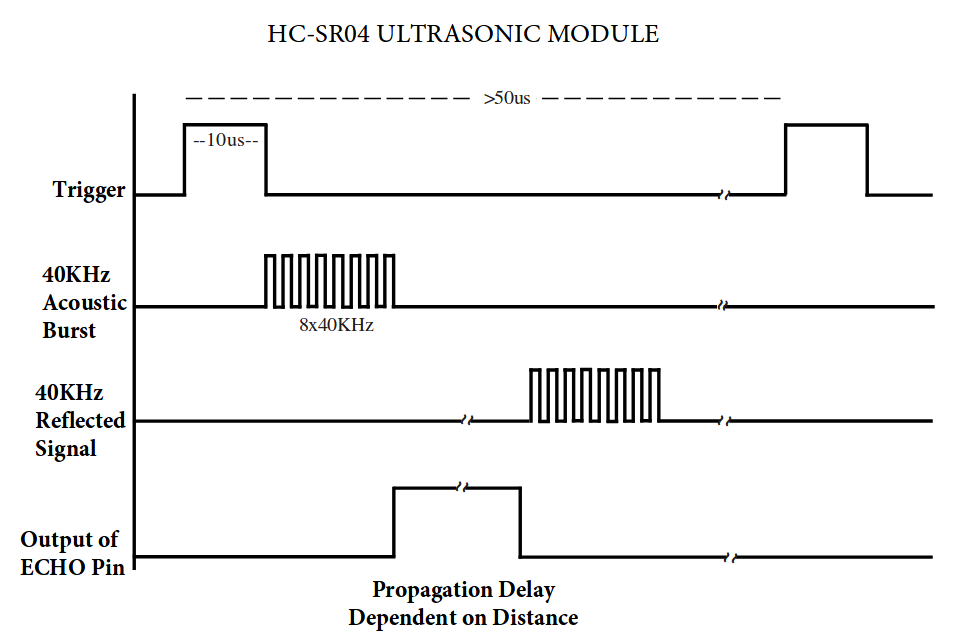
\includegraphics[width=.7\textwidth]{figs/8-hc-sr04-timing.png}

\paragraph{Coding:}

\begin{compactitem}[--]
\item To measure the duration of the pulse on the ECHO pin, we can use the
function \lstinline$pulseIn(pin, value)$:

\begin{tabular}{l | l}
  pin & the digital pin where the signal is connected (eg: ECHO) \\ \hline
  value & HIGH to measure the duration of the interval the signal is
  HIGH \\
  & LOW to measure the duration of the interval the signal is LOW
  \\ \hline
  return value & duration in $\mu$s ($10^{-6}$ sec). 
\end{tabular}

\item For the speed of sound, you can 
  use $331.5$ m/s at 0 deg Celsius. Add 0.6 m/s for each degree Celsius
  above 0. A typical room temperature is 20 degrees Celsius.

\item  Program: set the trigger signal like in the figure (make sure the
  trigger pulse is preceded by a 40 $\mu$s period when the signal is
  low. Immediately after generating the trigger pulse, measure the
  pulse on the ECHO line. Use the speed of sound to determine the
  distance.

\item  To generate pulses of the order of microseconds, one cannot use
  the \lstinline$delay()$ function like in Chapter
  \ref{lab1.ch}. However, a similar function does exactly what we
  need: it pauses the execution of the program for thr number of
  microseconds passed as its argument:

  \lstinline$delayMicroseconds(n)$: will pause the program for $n$
  microseconds, where $n$ is an unsigned integer.
\end{compactitem}

A sample program that outputs the measurements taken by the distance sensor is provided below.

\lstinputlisting[caption={Reading distance measurements from the distance sensor}]{src/distance.ino}


\section{Using the light sensors}

Two light sensors can be used to detect the direction for a source of
light.  Fasten the two sensors together, but separate them by a
protruding sheet of paper (see Fig.~\ref*{fig:2eyes}).  If the sensors
receive the same amount to light, it means the source of light is in
front of the pack of light sensors. If the source of light is to the
left of the pack of sensors, then the sensor on the left will measure
a more intense light than the sensor on the right because the sheet
of paper creates a shadow. This information can be used to rotate the
robot in the appropriate direction until the source of light is in
front of the robot.

For your program, consider using the advanced programming techniques described in class. Define a class that maintains the difference between the measurements from
the left and the right sensors.

\begin{figure}[tb]
  \begin{center}
	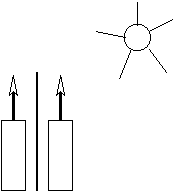
\includegraphics[width=.2\textwidth]{figs/2eyes}
  \end{center}
\caption{Light sensors to detect the direction of
  light.}	\label{fig:2eyes} 
\end{figure}


%%%%%%%%%%
\section{Programming and connecting the light and sound sensors}

\begin{figure}[tb]
  ~
  \hfill
  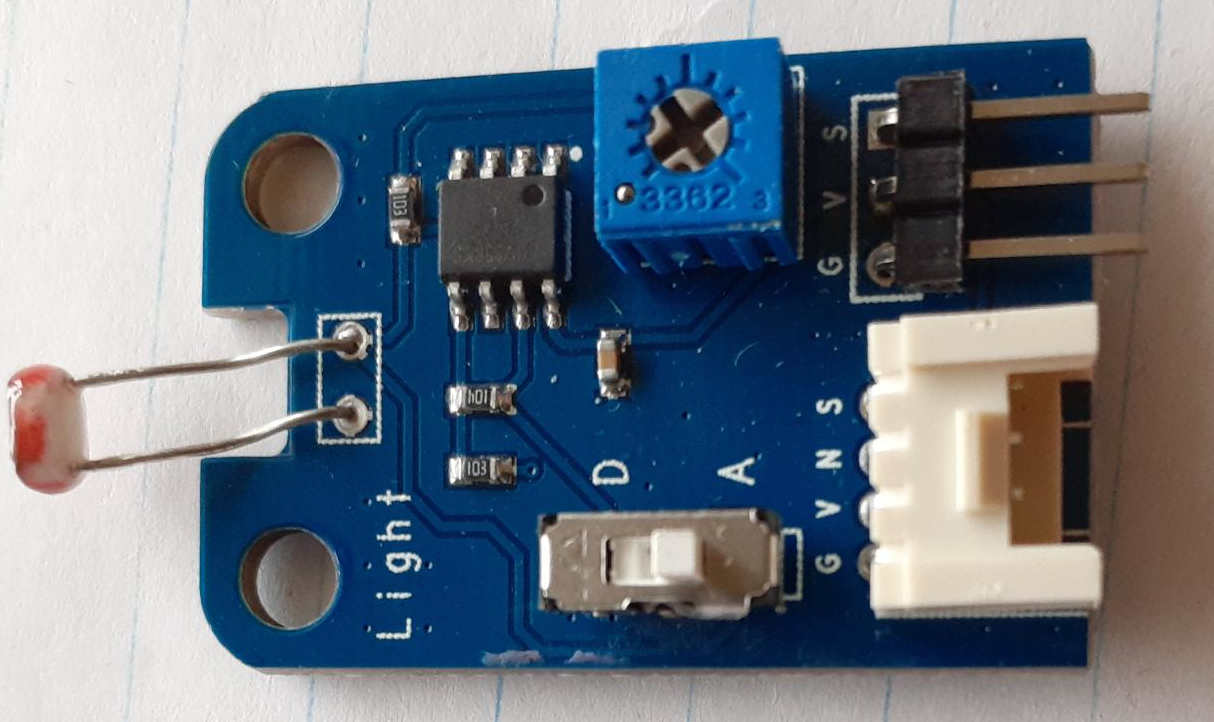
\includegraphics[width=.4\textwidth]{figs/light.jpg}
  \hfill
  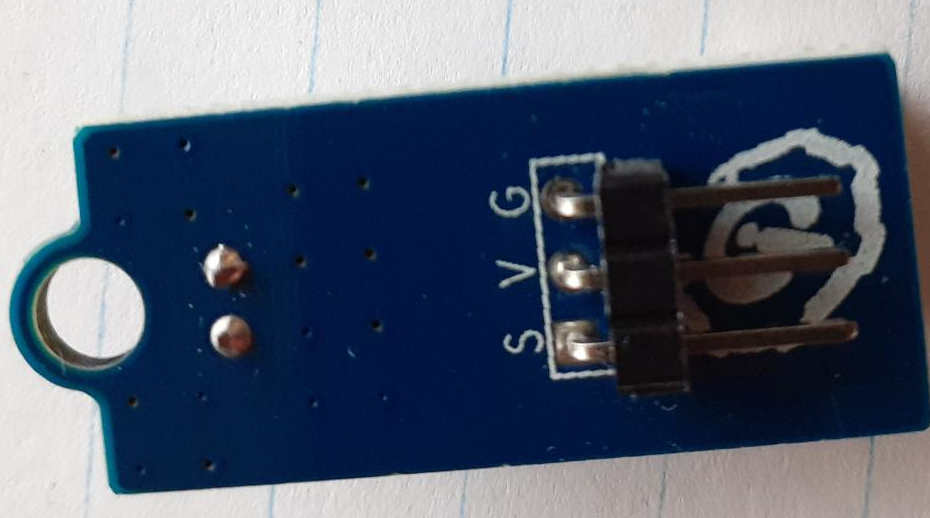
\includegraphics[width=.3\textwidth]{figs/sound.jpg}
  \hfill
  ~
  \caption{Left: light sensor. Right: the back of the sound sensor}\label{fig:light-sound}
\end{figure}

The light and sound sensors we are using are very simple sensors that generate analog signals. Please use the code from Section \ref{se:pot} that reads a general analog signal to experiment with these sensors.

\paragraph{The light sensor:} Examine Fig.~\ref{fig:light-sound}. The connection is simple. Use the group of black pins on the top with a female to female wire and connect as follows.

\smallskip
\begin{tabular}{c c}
  \toprule
  Sensor pin label & Arduino pin \\ \midrule
  V & 5 V \\
  G & GND \\
  S & one of A0-A5 \\ \bottomrule
\end{tabular}
\smallskip

The light sensor can be configured in digital mode, too. Notice the white switch in the figure. Make sure the switch is moved towards label A (analog mode). When in digital mode (switch towards label D) the blue potentiometer  defines a reference level. Any analog signal below this reference generates a digital LOW signal on the D pin, and any analog signal higher than the reference generates a HIGH digital signal on the digital pin D. The potentiometer can be turned using a Phillips screwdriver.

For this project, it is probably simpler to only use analog mode. However, if you feel that digital mode works better for your project, you are welcome to use it.

\paragraph{The sound sensor:} The sound sensor is simpler than the light sensor as it has no digital mode. The connections, as expected are identical with the connections for the light sensor (see the table above).


%%%%%%%%%%%%%%%%%%%%%%%%%

\appendix
\chapter{Revision history}

\begin{description}
\item[v 2.0:] Compared to version 1.0, Activity 0 was added and the
  order of activities was changed to improve the flow.
\item[v 2.1:] Exercise \ref{pb-sensor} from Chapter \ref{ch2.chap} was
  added.
\item[v 2.2:] The lab activity from Chapter \ref{se:ch4} was
  simplified and the original activity was assigned as an exercise,
  and new exercises were added.
\item[v 2.3:] Exercise \ref{prob5:grad} on page \pageref{prob5:grad}
  was revised and simplified.
\item[v 2.4] The code for the activity from Chapter \ref{ch:ex5} was
  simplified. Two exercises were added.
\item[v 3.0] Part II completely revised. Project challenges introduced.

\item[v 3.1.0] Part II: additional challenges introduced. Introduced a \emph{fast} stream with only two challenges instead of three. Removed the project log requirement.

  \item[v 3.1.1] Part II: added information about programming and connecting the sound and light sensors in the projects.
  
\end{description}
 
\end{document}
